\section{Requirements}

\section{Design}

\subsection{Background}
As with most software industries, when the paradigm of programming of software designs shifted from procedural and function-oriented programming to object-oriented programming, the game development industry adopted this change to take advantage of the many benefits that it offered. These benefits included data encapsulation, easier mapping of concepts to programming structures, and the ability to group and share behavior amongst objects of the same functional type. These benefits allowed additional functionality to be inserted without the need to duplicate a lot of code, thus greatly reducing the time, effort, and cost of developing large-scale software products.

\begin{figure}[h!]
  \centering 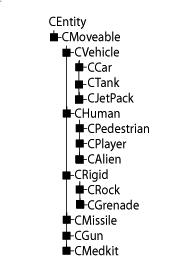
\includegraphics[width=0.2\textwidth]{Images/tree}
  \caption{A typical game object hierarchy. Source: http://cowboyprogramming.com/images/eyh/Fig-1.gif}
\end{figure}

In a typical object-oriented software product, the objects form a hierarchical tree that has width (many objects with the same direct ancestor, such as there are many weapon-types that are each modeled as an object, and they would all share the same ancestor of 'Weapon'.), and height (set of objects that form a list of direct ancestors for each other, such as how a 'DwarfMale' is a 'Dwarf' that is a 'PlayableCharacter' that is a 'Character' that is an 'Entity', and so on). This tree-like structure describes the term inheritance, where one object such as 'DwarfMale' may inherit functionality from 'Dwarf'. In small-to-medium sized products, inheritance can make development both simpler and much more efficient. However, as projects grow and changes are made, designing objects around inheritance can lead to problems due to relationships between objects in the tree. Changing or adding code at the root of the tree may cause the changes to cascade down through the rest of the tree, resulting in undesired behavior, as described by Herb Marslas, a developer for Age of Empires II:

\begin{quote}
\ldots functionality can be added or changed in a single place in the code to affect many different game units. One such change inadvertently added line-of-sight checking for trees.
\end{quote}

With the development archetype shifting from the waterfall method, where projects are defined at the beginning and are less adaptable to changes, to a more agile and iterative-based approach, the ability to change the project on both small and large scales becomes a requirement of the design of the project. As teams in the game development industry began to conduct agile development processes, they began to realize that the object-oriented design paradigm was not as flexible and adaptable as it needed to be, largely in part due to the inheritance structure and requirement of defined interfaces between objects.

To solve the issues with large inheritance trees, architects, designers, and programmers discovered the benefits of composition over inheritance, where it is better and/or easier to consider a has-a relationship over an is-a relationship. An example of this can be described as the difference between a 'Character' object having a position in the world, rather than a 'Character' object being a 'PositionalObject'. The distinction is small conceptually, but rather large in terms of design and implementation of the project. In order to change the 'Character' to not having a position, a developer would simply have to remove the position in regards to the composition method, while the inheritance method would require the object to be placed somewhere else in the tree, potentially leading to side effects and/or undesired behavior.

The realization of the benefits of composition over inheritance began a movement of the game development industry to a design pattern known as 'Entity-Component Systems', where objects are modelled by what they are composed of or contain, rather than their position in the hierarchical inheritance tree.

\subsection{Entity-Component Design}

\begin{figure}[h!]
  \centering 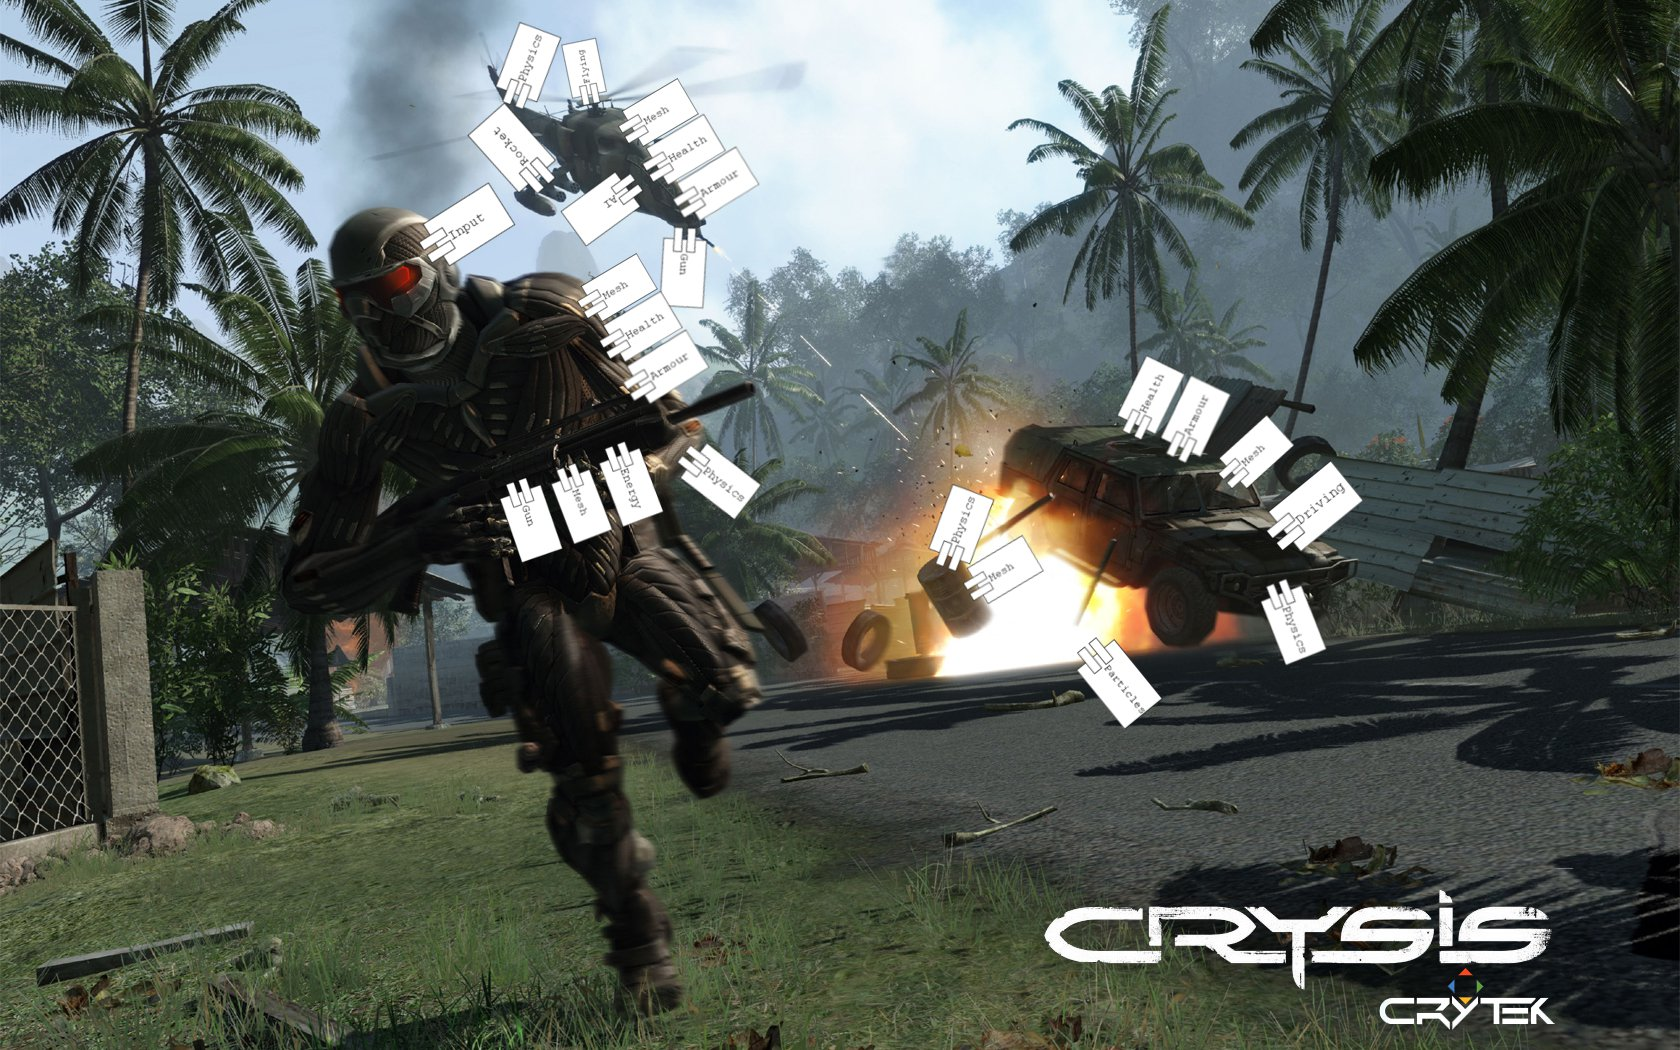
\includegraphics[width=0.48\textwidth]{Images/crysis-components.jpg}
  \caption{Entity component modelling in Crysis. Source: http://piemaster.net-content.s3.amazonaws.com/wp-content/uploads/crysis-components.jpg}
\end{figure}

The entity-component design paradigm is primarily focused on three primary objects in the application: entities, components, and system-managers (or component-managers). Entities are the primary conceptual objects in the game, such as 'Player', 'Target', and 'Map', among others. Components, on the

other hand, are essentially atomic parameters that can be attributed to an entity. For example, a 'Player' entity may have a 'Position' component, a 'Render' component, a 'Velocity' component, a 'Physics' component and anything else that describes the behavior of a 'Player' entity. The other object type, system-managers are objects responsible for the management of entities and their components, and the coordination and synchronization of each respective type. For example, a 'RenderSystemManager' may be responsible for iterating through every entity with a 'Render' component, and rendering that entity to the display.

There are many benefits that this type of design provides. The primary benefit, however, may be the fact that this type of design is inherently agile in nature. Changing the system is simply the process of adding, removing, or editing the desired entities and/or components. For example, to create a hidden trap object, an invisible object in the game that reacts in some way to the player, a developer may simply have to create the 'Trap' entity, provide it with a 'Position' component, and a 'Script' component that provides some behavioral functionality based on the 'Position' of the entity relative to the player, and register the entity with the correct system-manager that can update the 'Script' component whenever the player moves. Or to make the player invisible, a developer could simply remove the 'Render' component from the 'Player' entity. Additionally, once a component has been created, it is possible to reuse the component across the rest of the system or in future projects as it is simply a set of parameters containing no side-effects or requesting any interfaces for any other objects.

\begin{figure}[h!]
  \centering 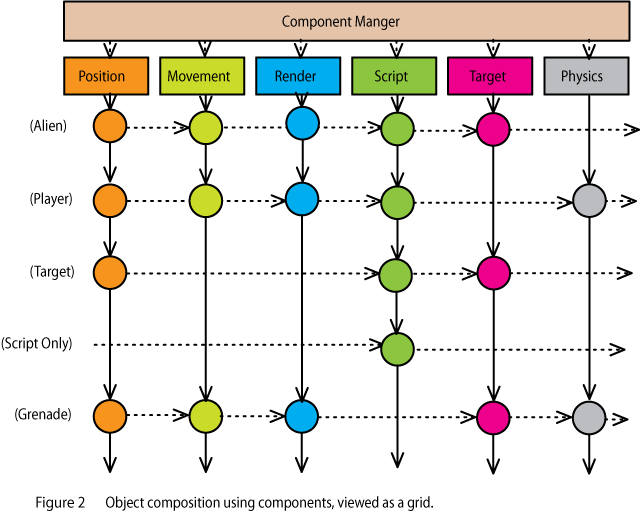
\includegraphics[width=0.5\textwidth]{Images/aggregation.png}
  \caption{Entity-component relationship. Source: http://cowboyprogramming.com/images/eyh/Fig-2.gif}
\end{figure}

Looking at this type of design, it is clear that the system and all of its entities are data-driven in nature. Rather than an object inheriting from some 'Renderable' object, the desire to render the object is encapsulated into whether or not the entity has a 'Render' component. With this in mind, the complimentary relationship between agile development and entity-component design actually increases

due to the fact that rather than having to receive requirements from a customer (the game designer, in respect to the game developer), the developer may actually allow the customer themselves to implement the desired functionality through a scripting engine, such as Dungeon Seige's scripting language Skrit.

\begin{figure}[h!]
  \centering 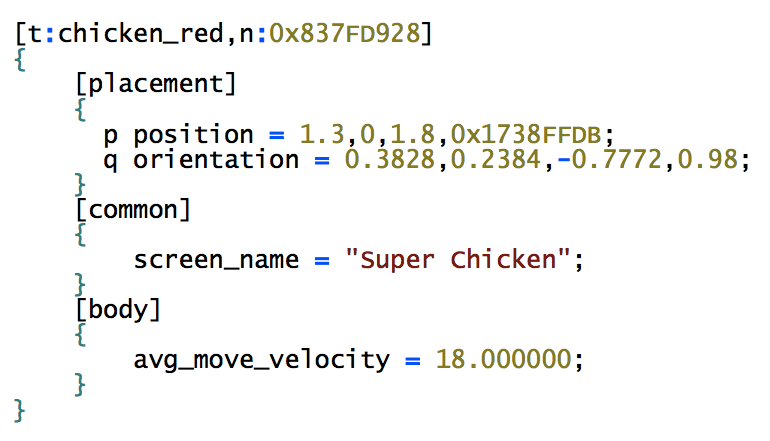
\includegraphics[width=0.4\textwidth]{Images/skrit.png}
  \caption{The Skrit scripting language for describing components. Source: http://scottbilas.com/files/2002/gdc\_san\_jose/game\_objects\_slides.pdf}
\end{figure}

Incorporating scripting languages allows the game designers--that is, the department whose job it is to define the functionality of the game and its entities--to actually define the functionality of an entity. Not only does this align perfectly with the agile manifesto, where interaction with the customer is paramount, but it also (if implemented correctly) allows different entity and components to be injected, removed, or edited at run-time to provide instant feedback to both the developer and the designer. This allows for an efficient iterative approach to be taken when developing the game as a whole.

The combination of entity-component systems with built-in scripting engines has become the primary design paradigm of modern game development, as showcased by the primary free, open source, and production game engines in the market today such as the Unreal Development Kit with Unrealscript scripting, and Unity3D with Mono, C\#, and Javascript scripting.

\subsection{Future of Game Design}

With the increased practice of agile development methodologies, and the realization of its complimentary nature with entity-component design with embedded scripting, it is likely that entity-component systems will continue to be the primary design archetype for the foreseeable future. So where does the industry go from here? A good modification candidate to the current methodology appears to be incorporating functional programming considerations within the game design. Functional programming is a programming method that strives for pure, non-state mathematical functions. Simply speaking, a pure function is a function that receives some input, performs some calculations, and returns a result or a modified copy of the input. A pure function is never able to access any state outside of the function's local scope. This is in stark contrast to the current paradigm of imperative programming, where typically it is the state of the application or an object that determines how the application behaves, with the goal of most functions to put the object or application into some known state.

Functional programming was originally introduced with LISP in the 1950s, but was slowly overshadowed by imperative programming due to the lack of computational resources to facilitate pure functional programming in performance-critical applications. However, as innovations in the number of transistors able to be packed onto a single processing chip has began to slow, processors have begun to incorporate additional parallel cores to increase processing power capabilities. With this plateau in processing power per core, and an increasing number of available cores, it is necessary for software to take advantage of parallel, multithreaded computing. However, the current method of imperative programming where application behavior is primarily driven by objects modifying state begins to break down in parallel environments as you begin to require transaction-based state modifications which can impose performance-limiting overhead. Thus, with parallel architectures becoming much more common, a paradigm-shift back to functional programming begins to provide tantalizing benefits.

While functional-versus-imperative programming is primarily an implementation-level decision, understanding the advantages and limitations of functional programming at a design-level may provide a better design in which to implement the specific programming archetype. Additionally, understanding that pure-functions do not interact with program state and do not produce any side effects allows functionality to be created iteratively in an agile approach. It is simply a matter of replacing a pure-function with a new implementation--say a better algorithm or different behavior altogether--and the rest of the code (in terms of program state) is unaffected by unsuspected side effects. With the nature of the code being simpler due to the reduced complexity of program state, the application becomes much easier to maintain and extend.

\section{Testing}

\section{Creative Interaction}

\section{Frameworks}
